\section{Convolution Neural Network} \label{sec:build5}

Convolution Neural Network [CNN Paper] combine different architectural ideas to ensure  shift and distortion invariances. In the Figure \ref{fig:Figure19} below it  can be seen that the input plane receives images that are approximately size-normalized and centered. Each unit of a layer receives input from units which are located locally in the previous layer. With local fields, it becomes easier for the neurons to extract visual features such as oriented edges, corners etc, these features are then combined by the higher layer called feature maps. It is being stated that distortion or shift in inputs causes the position of the salient features to vary. 

\begin{figure}[t]
	\DeclareGraphicsExtensions{.pdf,.png,.jpg}
	\begin{center}
		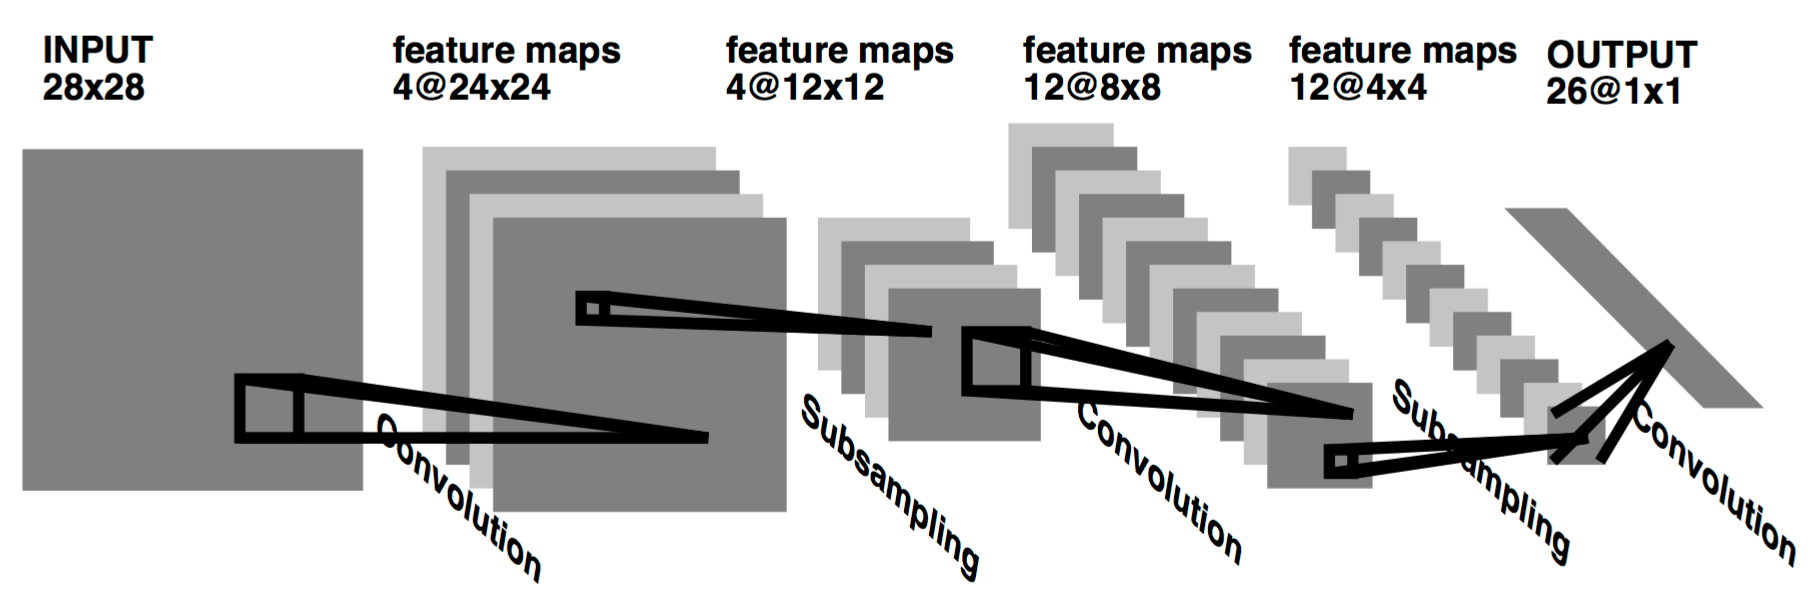
\includegraphics[width=\textwidth]{Figures/Figure19}
	\end{center}
	\caption{Typical CNN Network}
	\label{fig:Figure19}
\end{figure}


At each position, different types of units in different feature maps compute different types of features. A convolution layer is usually composed of several feature maps and as a matter of fact multiple features can be extracted at each location. The hidden layer in Figure \ref{fig:Figure19} has 4 feature maps with 5 by 5 receptive fields. Shifting the input of a convolution layer will shift the output. After detecting a feature, its location becomes less important as long as its relative position to other features is preserved. Thus, each convolution layer is followed by an additional layer while is called the pooling layer and it performs the subsampling and local averaging, thereby reducing the resolution of the feature map which reduces the effect to shifts and distortions. The second layer performs a 2 X 2 averaging and subsampling, followed by a trainable coefficient, a trainable bias , and a bias. The trainable coefficient and bias controls the effect of non-linearity. Then alternating layers of subsampling and convolutions are created successively where at each layer the number of feature maps are increased but the spatial resolution is decreased. The feature maps are then connected to form a fully-connected layer which is being fed into the softmax regression layer for classification purposes. All the weights are learned in the respective layers with back-propagation.

In recent times, Convolution Neural Networks(CNNs) have almost been used in all applications ranging from the popular ImageNet Large Scale Visual Recognition Challenge(ILSVRC) to various Recognition algorithms. It has taken the computer vision society by storm, improving the state of the art in many applications. Tremendous results have been obtained in tremendous large scale databases in recent times. \\

\textbf{ReLU Non-Linearity - } In CNNs, the standard way to model a neuron's output f as a function of of its input \textit{x} is with \textit{f(x) = tanh(x)} or \textit{f(x) = $(1+e^{-x})^{-1}$} . The training time with gradient descent algorithm is much slower due to saturation and nonlinearities thus a new concept can be applied here with non saturating neurons with nonlinearities where \textit{f(x) = max(0,x)}. These nuerons are known as Rectified Linear Units(ReLUs). CNNs with ReLUs train muc faster than their corresponding tanh units. The performance of the neurons also doesnot decrease as proven with experiments by Hinton and Nair[Hinton and Nair paper]. 

\begin{figure}
	\DeclareGraphicsExtensions{.pdf,.png,.jpg}
	\begin{center}
		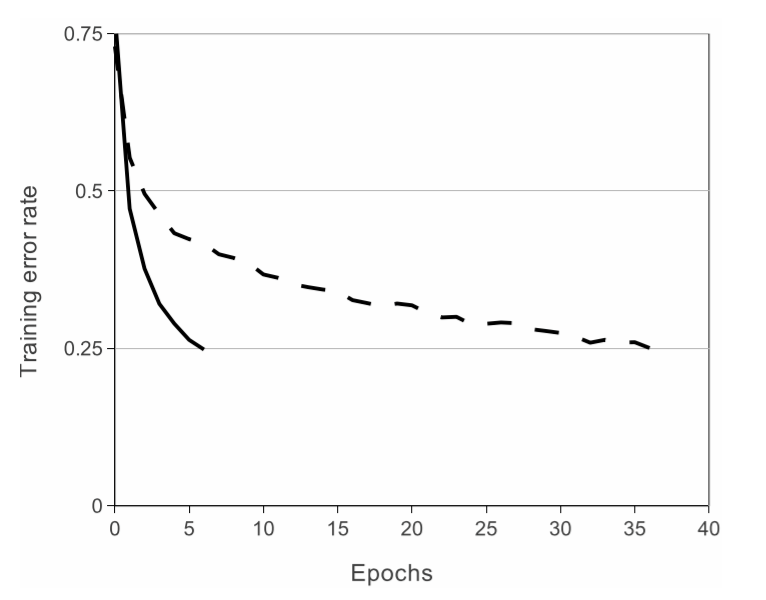
\includegraphics[width=0.5\textwidth]{Figures/Figure21}
	\end{center}
	\caption{Performance of a 4-layer ReLU CNN}
	\label{fig:Figure21}
\end{figure}

Figure \ref{fig:Figure21} [AlexNet paper] shows the number of iterations required to reach 25 p.c. training error on the CIFAR-10 dataset for a four layer convolution network. Thus it can be shown that faster learning has a great influence on the performance of large models which are trained on large datasets.

Another important concept to reduce test errors is the dropout technique. It seems to be too expensive for the big CNNs to train, which take several days to complete even on GPUs. The dropout technique consists of setting to zero the output of each hidden neuron with 50 p.c. probability, the dropped out neurons do not contribute to the forward pass and also do not participate in back-propagation approach. So every time, the neural network samples a different architecture but all the architecture share weights. This technique educes the complex o-adaptations of neurons since a neuron cannot rely on the presence of particular other neurons.It is, therefore, forced to learn more robust features that are useful in conjunction with many different random subsets of the other neurons. At test time, we use all the neurons but multiply their outputs by 0.5, which is a reasonable approximation to taking the geometric mean of the predictive distributions produced by the exponentially-many dropout networks.

Dropout is mostly applied to the Fully-connected layer in a CNN. Dropout helps to prevent overfitting in a neural networknd thus is an extremely useful concept.



